\section{Usecase diagram}
\subsection{Toàn bộ hệ thống}
\begin{figure}[H]
    \centering
    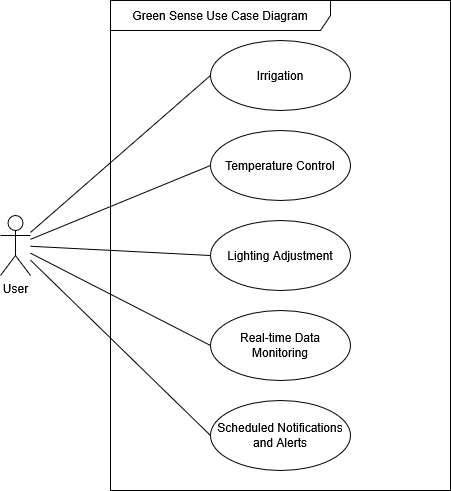
\includegraphics[width=0.85\linewidth]{content/images/Use Case Diagram.png}
    \caption{Biểu đồ use case cho hệ thống Green Sense}
    \label{fig:useCaseDiagram}
\end{figure}
\subsection{Bảng mô tả cho từng use case}
\subsubsection{Use case 1 - Tưới nước}
TBU
% \renewcommand{\arraystretch}{1.6}
% \begin{table}[H]
% \centering
% \begin{tabular}{|p{0.2\linewidth}|p{0.7\linewidth}|}
% \hline
% \rowcolor[HTML]{EFEFEF} 
% \textbf{Usecase}        & \textbf{Tưới nước} \\ \hline
% Use case ID             & 1 \\ \hline
% Actor                   & Người dùng của hệ thống \\ \hline
% Description             & Lorem ipsum dolor sit amet, consectetur adipiscing elit. Nulla ut augue in odio ultricies vehicula vel quis ex. Nullam ut lacinia ex, eget maximus ante. Donec dictum rutrum efficitur. Aliquam ut dui in nunc tincidunt posuere eget vitae arcu. In eget leo id turpis scelerisque malesuada. Nam semper fringilla lorem nec ornare. Mauris gravida pharetra enim, at fermentum nunc. \\ \hline
% Precondition            & Sed laoreet ultrices lobortis. Proin pretium aliquet neque vel suscipit. Nam nec auctor sem. Orci varius natoque penatibus et magnis dis parturient montes, nascetur ridiculus mus. Maecenas tincidunt at erat porta lobortis. Aenean a tincidunt erat. Integer tempus orci a ornare feugiat. Cras eros ligula, laoreet et ante eu, consectetur lacinia mi. Cras ac porttitor ex, id facilisis tortor. Duis sit amet auctor enim. \\ \hline
% Postcondition           & Vivamus luctus lacinia ullamcorper. Fusce a fermentum nunc. Quisque luctus lobortis dolor id blandit. Donec quis tortor volutpat, vehicula lectus ac, dictum magna. Sed in sem non nisi finibus finibus. Etiam sagittis nisl sit amet urna ultrices condimentum. Donec nec molestie ligula. Vestibulum pellentesque feugiat lacus vel gravida. Vivamus sed egestas nisl. Praesent lacus  Fusce viverra purus quis eleifend gravida.  \\ \hline
% Trigger                 & Vivamus luctus lacinia ullamcorper. Fusce a fermentum nunc. Quisque luctus lobortis dolor id blandit. Donec quis tortor volutpat, vehicula lectus ac, dictum magna. Sed in sem non nisi finibus finibus. Etiam sagittis nisl sit amet urna ultrices condimentum. Donec nec molestie ligula. Vestibulum pellentesque feugiat lacus vel gravida. Vivamus sed egestas nisl. Praesent lacus  Fusce viverra purus quis eleifend gravida.  \\ \hline
% Normal Flow             & Vivamus luctus lacinia ullamcorper. Fusce a fermentum nunc. Quisque luctus lobortis dolor id blandit. Donec quis tortor volutpat, vehicula lectus ac, dictum magna. Sed in sem non nisi finibus finibus. Etiam sagittis nisl sit amet urna ultrices condimentum. Donec nec molestie ligula. Vestibulum pellentesque feugiat lacus vel gravida. Vivamus sed egestas nisl. Praesent lacus  Fusce viverra purus quis eleifend gravida.  \\ \hline
% Exception Flow          & Vivamus luctus lacinia ullamcorper. Fusce a fermentum nunc. Quisque luctus lobortis dolor id blandit. Donec quis tortor volutpat, vehicula lectus ac, dictum magna. Sed in sem non nisi finibus finibus. Etiam sagittis nisl sit amet urna ultrices condimentum. Donec nec molestie ligula. Vestibulum pellentesque feugiat lacus vel gravida. Vivamus sed egestas nisl. Praesent lacus  Fusce viverra purus quis eleifend gravida.  \\ \hline
% \end{tabular}
% \caption{Usecase specification ABC}
% \end{table}

\subsubsection{Use case 2 - Điều chỉnh nhiệt độ}
\renewcommand{\arraystretch}{1.6}
\begin{table}[H]
\centering
\begin{tabular}{|p{0.2\linewidth}|p{0.7\linewidth}|}
\hline
\rowcolor[HTML]{EFEFEF} 
\textbf{Usecase}        & \textbf{Điều chỉnh nhiệt độ} \\ \hline
Use case ID             & 2 \\ \hline
Actor                   & Người dùng của hệ thống \\ \hline
Description             & 
    Với tính năng kiểm soát nhiệt độ, hệ thống cung cấp 3 lựa chọn:
    \begin{itemize}
        \item [--] \textbf{Chế độ tự động:} Hệ thống cố gắng duy trì nhiệt độ bên trong nhà kính ở mức lý tưởng.
        \item [--] \textbf{Chế độ theo lịch:} Tuân theo lịch trình mà người dùng cài đặt (theo ngày, tuần hoặc tháng), kèm theo tùy chọn dự phòng an toàn (nếu muốn) để hệ thống tự điều chỉnh khi có biến động bất thường.
        \item [--] \textbf{Chế độ thủ công:} Người dùng toàn quyền điều khiển đóng/mở các tấm che nắng (là những tấm che trên trần có khả năng cản sáng; trong mô hình này, chúng ta dùng động cơ mô phỏng việc cuốn/mở tấm che), bất cứ khi nào họ muốn.
    \end{itemize}
\\ \hline
Precondition            & 
Hệ thống đang vận hành bình thường. \newline
Hệ thống được trang bị cảm biến DHT20 để đo nhiệt độ và độ ẩm. \newline
Tùy chọn, hệ thống có lắp các tấm che nắng kết nối với bộ truyền động (Động cơ Servo SG90S) để cuộn vào hoặc mở ra. 
\\ \hline
Postcondition           & 
Nhiệt độ (đo bởi cảm biến) và trạng thái của tấm che nắng được ghi nhận vào cơ sở dữ liệu của hệ thống theo định kỳ. \newline
Mọi hành động điều chỉnh nhiệt độ (do người dùng thực hiện hoặc do hệ thống tự động) đều được ghi lại vào lịch sử.
\\ \hline
Normal Flow             & 
1. Người dùng mở ứng dụng di động. \newline
2. Người dùng chọn “Temperature control” (Kiểm soát nhiệt độ) từ danh sách tính năng trên màn hình chính. \newline
3. Người dùng chọn “Scheduled mode” (Chế độ theo lịch). \newline
4. Người dùng thiết lập chế độ dự phòng an toàn thành “do nothing” (không làm gì), “warn” (chỉ cảnh báo) hoặc “warn and take action” (cảnh báo và tự xử lý). \newline
5. Hệ thống cung cấp một thanh trượt (slider) theo dải thời gian 24 giờ trong ngày. \newline
6. Người dùng chọn khung giờ mong muốn để tấm che nắng mở hoặc đóng.
\\ \hline
Alternative Flow 1        & 
3.1. Tại bước 3, nếu người dùng chọn “Automatic” (Tự động): \newline
3.1.1 Người dùng chỉ định khoảng nhiệt độ mục tiêu. \newline
3.1.2 Hệ thống bắt đầu kiểm tra mức nhiệt mỗi khi có dữ liệu mới từ cảm biến. Ví dụ, nếu nhiệt độ bên trong nhà kính thấp hơn khoảng mục tiêu từ 3 đến 5 độ C, hệ thống sẽ mở các tấm che nắng cho đến khi nhiệt độ đo được nằm trong khoảng đã thiết lập.
\\ \hline
Alternative Flow 2        & 
3.2. Tại bước 3, nếu người dùng chọn “Manual” (Thủ công): \newline
3.2.1 Người dùng chỉ định xem hệ thống có nên gửi cảnh báo khi nhiệt độ nguy hiểm hay không. \newline
3.2.2 Nếu bật cảnh báo, hệ thống thường xuyên giám sát nhiệt độ và có thể gửi thông báo khi nhiệt độ vượt quá ngưỡng an toàn.
\\ \hline
\end{tabular}
\caption{Bảng mô tả cho use case Điều chỉnh nhiệt độ}
\end{table}

\subsubsection{Use case 3 - Điều chỉnh ánh sáng}
\renewcommand{\arraystretch}{1.6}
\begin{table}[H]
\centering
\begin{tabular}{|p{0.2\linewidth}|p{0.7\linewidth}|}
\hline
\rowcolor[HTML]{EFEFEF} 
\textbf{Usecase}        & \textbf{Điều chỉnh ánh sáng} \\ \hline
Use case ID             & 3 \\ \hline
Actor                   & Người dùng của hệ thống \\ \hline
Description             & Chúng ta có thể tùy chỉnh cho phù hợp các mức độ ánh sáng phù hợp trong nhà trồng cây với 3 chế độ: tự động điều chỉnh phù hợp với điều kiện môi trường, lập lịch các khoảng thời gian trong ngày hoặc các ngày trong tuần, hoặc người dùng có thể điều chỉnh ánh sáng của đèn trực tiếp. Hệ thống có cũng có thể cảnh báo về vấn đề đèn bị hư hỏng hoặc mức độ sáng không phù hợp nằm ngoài khả năng điều chỉnh của hệ thống. \\ \hline
Precondition            & Hệ thống hoạt động bình thường và luôn được trang bị cảm biến ánh sáng và một mạch role gắn vào nguồn chiếu sáng của nguồn chiếu sáng. \\ \hline
Postcondition           & Mức độ ánh sáng được đo bằng cảm biến và cấu hình hệ thống chiếu sáng được lưu vào cơ sở dữ liệu của hệ thống sau mỗi nửa tiếng. Các hành động điều chỉnh mức độ sáng bởi người dùng hay hệ thống đều được lưu vào lịch sử theo dõi. \\ \hline
Normal Flow             & 
    1. Người dùng mở ứng dụng di động. \newline
    2. Người dùng chọn ``Điều chỉnh chế độ sáng" từ danh sách các tính năng trên màn hình chính. \newline
    3. Người dùng chọn ``Lập lịch". \newline
    4. Người dùng thiết lập một chế độ dự phòng bao gồm: ``Không hành động", ``Cảnh báo", ``Cảnh báo và hành động". \newline
    5. Hệ thống cung cấp một thanh trượt dựa trên phạm vi biểu thị 24h trong ngày. \newline
    6. Người dùng chọn khoảng thời gian mong muốn trong ngày để đèn hoạt động. 
  \\ \hline
Alternative Flow 1          & 
    3.1. Ở bước 3, nếu người dùng chọn `Tự động' trên thanh tùy chọn: \newline
    3.1.1. Người dùng chọn cụ thể mức độ sáng mục tiêu \newline
    3.1.2. Hệ thống bắt đầu kiểm tra và nhận dữ liệu về sau mỗi đơn vị thời gian. Nếu mức độ sáng không phù hợp với cấu hình không đúng với mục tiêu, hệ thống sẽ điều chỉnh đến khi nào cảm biến ánh sáng nhận được dữ liệu với mức độ sáng phù hợp với cấu hình   \\ \hline
Alternative Flow 2          & 
    3.2. Ở bước 3, nếu người dùng chọn `Thủ công' trên thanh tùy chọn: \newline
    3.2.1. Người dùng chọn cụ thể những gì hệ thống nên cảnh báo ví dụ như mức sáng thấp, hay khả năng xảy ra hư hỏng hệ thống chiếu sáng. \newline
    3.2.2. Nếu cảnh báo được bật, hệ thống sẽ giám sát mức độ ánh sáng thường xuyên và có thể cảnh báo thông qua thiết bị người dùng. \\ \hline
\end{tabular}
\caption{Bảng mô tả cho use case Điều chỉnh ánh sáng}
\end{table}

\subsubsection{Use case 4 - Theo dõi dữ liệu theo thời gian thực và thống kê hệ thống}
\renewcommand{\arraystretch}{1.6}
\begin{table}[H]
\centering
\begin{tabular}{|p{0.2\linewidth}|p{0.7\linewidth}|}
\hline
\rowcolor[HTML]{EFEFEF} 
\textbf{Usecase}        & \textbf{Theo dõi dữ liệu theo thời gian thực và thống kê hệ thống} \\ \hline
Use case ID             & 4 \\ \hline
Actor                   & Người dùng của hệ thống \\ \hline
Description             & Ứng dụng cho phép người dùng xem dữ liệu đã ghi dưới dạng báo cáo tổng hợp (trong một khoảng thời gian) với các tính toán tổng hợp và biểu đồ tổng quan về các bản ghi trước đó. \\ \hline
Precondition            & Ứng dụng di động được kết nối với cơ sở dữ liệu và hệ thống vẫn đang ghi lại thống kê. \\ \hline
Postcondition           & Không có.  \\ \hline
Normal Flow             & 
    1. Người dùng mở ứng dụng di động. \newline
    2. Người dùng chọn `Thống kê' từ danh sách các tính năng trên màn hình chính. \newline
    3. Hệ thống trích xuất dữ liệu hàng ngày làm chế độ báo cáo mặc định và hiển thị cho người dùng. Báo cáo bao gồm biểu đồ đường về mức ánh sáng, độ ẩm và nhiệt độ trong khoảng thời gian đó; các hành động đáng chú ý được thực hiện thủ công hoặc tự động trên hệ thống nhà kính; và trạng thái mới nhất của nhà kính (các phép đo nhận được gần nhất). \newline
    4. Người dùng có thể chọn khoảng thời gian ưa thích bằng cách chọn `Khoảng thời gian' trên thanh tùy chọn. \newline
    5. Hệ thống cung cấp lịch chi tiết để người dùng chọn ngày bắt đầu và ngày kết thúc cho báo cáo. \newline
    6. Người dùng chọn khoảng thời gian ưa thích và nhấn `Xác nhận'. \newline
    7. Hệ thống tải lại trang báo cáo với chế độ hiển thị biểu đồ phù hợp và theo dõi hành động. \newline
    8. Người dùng nhấn `Hoàn tất' để quay lại trang chính.
\\ \hline
Alternative Flow          & 
Ở bước 3, nếu người dùng chọn `Thống kê để báo cáo' trên thanh tùy chọn: \newline
3.1. Hệ thống hiển thị danh sách dữ liệu để ghi nhận (mặc định, mọi tùy chọn đều được chọn) để người dùng chọn dữ liệu cần báo cáo. \newline
3.2. Người dùng chọn/bỏ chọn các mục phù hợp và nhấn `Xác nhận'. \newline
3.3. Hệ thống lưu cấu hình và chỉ báo cáo các mục đã chọn vào lần sau.
\\ \hline
Exception Flow          & 
Ở bước 4, khoảng thời gian mà người dùng chỉ định không có trong hệ thống cơ sở dữ liệu. \newline
4.1. Hệ thống hiển thị cửa sổ lỗi và đề xuất người dùng chọn một khoảng thời gian hợp lệ.  
\\ \hline
\end{tabular}
\caption{Bảng mô tả cho use case Theo dõi dữ liệu theo thời gian thực và thống kê hệ thống}
\end{table}

\subsubsection{Use case 5 - Cài đặt thông báo và cảnh báo theo lịch trình}
TBU
% \renewcommand{\arraystretch}{1.6}
% \begin{table}[H]
% \centering
% \begin{tabular}{|p{0.2\linewidth}|p{0.7\linewidth}|}
% \hline
% \rowcolor[HTML]{EFEFEF} 
% \textbf{Usecase}        & \textbf{Tưới nước} \\ \hline
% Use case ID             & 5 \\ \hline
% Actor                   & Người dùng của hệ thống \\ \hline
% Description             & Lorem ipsum dolor sit amet, consectetur adipiscing elit. Nulla ut augue in odio ultricies vehicula vel quis ex. Nullam ut lacinia ex, eget maximus ante. Donec dictum rutrum efficitur. Aliquam ut dui in nunc tincidunt posuere eget vitae arcu. In eget leo id turpis scelerisque malesuada. Nam semper fringilla lorem nec ornare. Mauris gravida pharetra enim, at fermentum nunc. \\ \hline
% Precondition            & Sed laoreet ultrices lobortis. Proin pretium aliquet neque vel suscipit. Nam nec auctor sem. Orci varius natoque penatibus et magnis dis parturient montes, nascetur ridiculus mus. Maecenas tincidunt at erat porta lobortis. Aenean a tincidunt erat. Integer tempus orci a ornare feugiat. Cras eros ligula, laoreet et ante eu, consectetur lacinia mi. Cras ac porttitor ex, id facilisis tortor. Duis sit amet auctor enim. \\ \hline
% Postcondition           & Vivamus luctus lacinia ullamcorper. Fusce a fermentum nunc. Quisque luctus lobortis dolor id blandit. Donec quis tortor volutpat, vehicula lectus ac, dictum magna. Sed in sem non nisi finibus finibus. Etiam sagittis nisl sit amet urna ultrices condimentum. Donec nec molestie ligula. Vestibulum pellentesque feugiat lacus vel gravida. Vivamus sed egestas nisl. Praesent lacus  Fusce viverra purus quis eleifend gravida.  \\ \hline
% Trigger                 & Vivamus luctus lacinia ullamcorper. Fusce a fermentum nunc. Quisque luctus lobortis dolor id blandit. Donec quis tortor volutpat, vehicula lectus ac, dictum magna. Sed in sem non nisi finibus finibus. Etiam sagittis nisl sit amet urna ultrices condimentum. Donec nec molestie ligula. Vestibulum pellentesque feugiat lacus vel gravida. Vivamus sed egestas nisl. Praesent lacus  Fusce viverra purus quis eleifend gravida.  \\ \hline
% Normal Flow             & Vivamus luctus lacinia ullamcorper. Fusce a fermentum nunc. Quisque luctus lobortis dolor id blandit. Donec quis tortor volutpat, vehicula lectus ac, dictum magna. Sed in sem non nisi finibus finibus. Etiam sagittis nisl sit amet urna ultrices condimentum. Donec nec molestie ligula. Vestibulum pellentesque feugiat lacus vel gravida. Vivamus sed egestas nisl. Praesent lacus  Fusce viverra purus quis eleifend gravida.  \\ \hline
% Exception Flow          & Vivamus luctus lacinia ullamcorper. Fusce a fermentum nunc. Quisque luctus lobortis dolor id blandit. Donec quis tortor volutpat, vehicula lectus ac, dictum magna. Sed in sem non nisi finibus finibus. Etiam sagittis nisl sit amet urna ultrices condimentum. Donec nec molestie ligula. Vestibulum pellentesque feugiat lacus vel gravida. Vivamus sed egestas nisl. Praesent lacus  Fusce viverra purus quis eleifend gravida.  \\ \hline
% \end{tabular}
% \caption{Usecase specification ABC}
% \end{table}


\newpage

% Table template %

% \renewcommand{\arraystretch}{1.6}
% \begin{table}[H]
% \centering
% \begin{tabular}{|l|l|}
% \hline
% \rowcolor[HTML]{EFEFEF} 
% \textbf{Usecase}          & \textbf{Usecase ABC} \\ \hline
% Actor            & Người dùng của hệ thống \\ \hline
% Description      & \begin{tabular}[c]{@{}l@{}}Mô tả chi tiết chức năng chính  \\ Mô tả chi tiết chức năng chính\end{tabular} \\ \hline
% Precondition     & \\ \hline
% Postcondition    & \\ \hline
% Trigger          & \\ \hline
% Normal Flow      & \\ \hline
% Exception Flow   & \\ \hline
% \end{tabular}
% \caption{Usecase specification ABC}
% \end{table}